% Options for packages loaded elsewhere
\PassOptionsToPackage{unicode}{hyperref}
\PassOptionsToPackage{hyphens}{url}
\documentclass[
  10pt,
]{article}
\usepackage{xcolor}
\usepackage[margin=22mm]{geometry}
\usepackage{amsmath,amssymb}
\setcounter{secnumdepth}{-\maxdimen} % remove section numbering
\usepackage{iftex}
\ifPDFTeX
  \usepackage[T1]{fontenc}
  \usepackage[utf8]{inputenc}
  \usepackage{textcomp} % provide euro and other symbols
\else % if luatex or xetex
  \usepackage{unicode-math} % this also loads fontspec
  \defaultfontfeatures{Scale=MatchLowercase}
  \defaultfontfeatures[\rmfamily]{Ligatures=TeX,Scale=1}
\fi
\usepackage{lmodern}
\ifPDFTeX\else
  % xetex/luatex font selection
    \setmainfont[]{DejaVu Serif}
\fi
% Use upquote if available, for straight quotes in verbatim environments
\IfFileExists{upquote.sty}{\usepackage{upquote}}{}
\IfFileExists{microtype.sty}{% use microtype if available
  \usepackage[]{microtype}
  \UseMicrotypeSet[protrusion]{basicmath} % disable protrusion for tt fonts
}{}
\makeatletter
\@ifundefined{KOMAClassName}{% if non-KOMA class
  \IfFileExists{parskip.sty}{%
    \usepackage{parskip}
  }{% else
    \setlength{\parindent}{0pt}
    \setlength{\parskip}{6pt plus 2pt minus 1pt}}
}{% if KOMA class
  \KOMAoptions{parskip=half}}
\makeatother
\usepackage{longtable,booktabs,array}
\usepackage{calc} % for calculating minipage widths
% Correct order of tables after \paragraph or \subparagraph
\usepackage{etoolbox}
\makeatletter
\patchcmd\longtable{\par}{\if@noskipsec\mbox{}\fi\par}{}{}
\makeatother
% Allow footnotes in longtable head/foot
\IfFileExists{footnotehyper.sty}{\usepackage{footnotehyper}}{\usepackage{footnote}}
\makesavenoteenv{longtable}
\usepackage{graphicx}
\makeatletter
\newsavebox\pandoc@box
\newcommand*\pandocbounded[1]{% scales image to fit in text height/width
  \sbox\pandoc@box{#1}%
  \Gscale@div\@tempa{\textheight}{\dimexpr\ht\pandoc@box+\dp\pandoc@box\relax}%
  \Gscale@div\@tempb{\linewidth}{\wd\pandoc@box}%
  \ifdim\@tempb\p@<\@tempa\p@\let\@tempa\@tempb\fi% select the smaller of both
  \ifdim\@tempa\p@<\p@\scalebox{\@tempa}{\usebox\pandoc@box}%
  \else\usebox{\pandoc@box}%
  \fi%
}
% Set default figure placement to htbp
\def\fps@figure{htbp}
\makeatother
\setlength{\emergencystretch}{3em} % prevent overfull lines
\providecommand{\tightlist}{%
  \setlength{\itemsep}{0pt}\setlength{\parskip}{0pt}}
% Draft layout: tables use the entire available text width via Pandoc colspecs.
\usepackage{microtype}
\usepackage{float}
\floatplacement{figure}{H}
\usepackage{fvextra}
\DefineVerbatimEnvironment{Highlighting}{Verbatim}{breaklines,commandchars=\\\{\}}
\setlength{\emergencystretch}{3em}
\sloppy
\AtBeginEnvironment{longtable}{\small}
\usepackage{bookmark}
\IfFileExists{xurl.sty}{\usepackage{xurl}}{} % add URL line breaks if available
\urlstyle{same}
\hypersetup{
  hidelinks,
  pdfcreator={LaTeX via pandoc}}

\author{}
\date{}

\begin{document}

\section{SOKKANAEM-Refresh: Toward Efficient Streaming Depth Estimation
for Fixed-View
Cameras}\label{sokkanaem-refresh-toward-efficient-streaming-depth-estimation-for-fixed-view-cameras}

\begin{quote}
Working draft, 10 September 2026. Target application fixed to indoor,
fixed-view cameras observing dynamic scenes. This scope was chosen after
a new moving-camera test failed short-clip quality; the failure is
retained. Existing experiments are mixed-camera evidence, not completed
fixed-camera validation. This is not submission-ready. The
\href{draft_native_20260909.md}{native-SSM draft} and original
\texttt{submission/manuscript.tex} are preserved. These speed results do
not belong to the 4.19M native model.
\end{quote}

\subsection{Authors and declarations}\label{authors-and-declarations}

Names, affiliations, correspondence, contributions, funding, conflicts
of interest, permissions and release arrangements will be completed and
verified by the authors. No external submission or public release is
implied.

\subsection{Abstract}\label{abstract}

We target indoor fixed-view cameras observing dynamic scenes, where
reduced camera-induced change motivates reuse but does not eliminate
object motion or disocclusion. This application hypothesis still
requires a fresh, verified fixed-camera evaluation; real-time deployment
is a target, not an established result.

Reusing estimated depth can reduce streaming inference cost, but motion
compensation and refresh decisions can consume the intended savings. We
investigate SOKKANAEM as a causal inference pipeline combining a frozen
depth predictor, transported depth caches and a lightweight pre-flow
refresh policy. The policy uses current-to-anchor RGB statistics and
cache age to decide whether to run the full predictor before paying
optical-flow cost. Accepted reuse nearest-warps the previous depth; full
refresh reproduces the frozen predictor. A 1,688-parameter MLP is
trained on a depth-and-gradient discrepancy proxy and compared with
similarly sized state-space policies. On reused TUM/Bonn development
clips of 32 and 256 frames, the selected MLP satisfies a fixed
multi-metric quality screen. Three timing repeats on a shared RTX 4090
give 3.762 ms/frame on the 256-frame clips, compared with 7.512 ms for
the dense predictor and 4.360 ms for fixed-period K2 reuse: a 13.73\%
latency reduction relative to K2. A one-frame initialization shift also
passes. However, the long-clip flat-region variation increase is
0.963\%, close to the 1\% tolerance. These findings support pre-flow
scheduling as a development-stage efficiency mechanism, not a general
accuracy guarantee, independently validated generalization result or
state-space memory advantage.

The subsequent frozen-candidate test on two newly acquired TUM sequences
passes the long-clip screen but fails the short-clip screen: aggregate
overshoot increases 2.285\%. Thus, the development speed--quality result
does not transfer uniformly to the new sequences.

\subsection{1. Introduction}\label{introduction}

A streaming depth system produces a dense map for each incoming frame. A
strong single-image estimator supplies detailed predictions, yet
evaluating every frame repeats expensive computation. Reuse trades
computation for approximation: cached depth must follow motion, and
transport errors may accumulate until refresh.

The question here is whether a learned policy can extend reuse beyond a
strong fixed-period K2 control without exceeding a stated quality
tolerance and while costing less. A decision that computes optical flow
and then rejects reuse can waste the computation it was intended to
save. We therefore place a compact RGB decision before flow.

We call the selected pipeline \textbf{SOKKANAEM-Refresh}, distinguishing
it from the earlier native SSM architecture. It preserves the expensive
depth estimator and changes when it runs. It does not introduce a new
monocular-depth backbone or use current ground-truth depth at inference.
Its investigated contributions are a causal pre-flow pipeline,
controlled fixed/learned and early/late decision comparisons, and a
reproducible development screen with exact-output audits and failure
visualizations. Temporal reuse itself is not claimed as a first
contribution.

\subsubsection{1.1. Fixed-view application
contract}\label{fixed-view-application-contract}

The primary application is monocular RGB streaming from an indoor camera
whose position, orientation and focal length remain fixed during a
recording. People and objects moving, entering or leaving the view,
occlusion, disocclusion and illumination changes remain in scope. A
fixed camera is not a static scene. Small camera vibration will be
reported separately as quasi-fixed sensitivity analysis; moving cameras,
PTZ and zoom are outside the primary application. Reconnection or a
known recording cut requires a new stream initialization; automatic cut
detection has not been implemented.

The expected benefit is reduced camera-induced variation, which may
permit more reuse. This is a mechanism-based hypothesis, not a measured
fixed-camera advantage. The current method schedules whole-frame Q0
calls and does not selectively recompute spatial regions. The frozen
checkpoint and threshold have not changed with the application scope. We
record that the narrowing occurred after observing the Section 6.6
failure, avoiding a retrospective claim of successful validation. The
full \href{streaming_draft/FIXED_CAMERA_SCOPE.md}{scope contract}
specifies inclusion rules and pending tests.

\subsection{2. Related work}\label{related-work}

Depth Anything V2 supplies the pretrained representation and decoder
{[}1{]}. Our Q0 reference combines its Small model with an existing
locally trained metric-calibration head. The reference's pretrained
shape quality is not a contribution of the refresh policy. Dense Inverse
Search (DIS) supplies the optical-flow method {[}2{]}. Eventful
Transformers exploit temporal redundancy within transformer computation
{[}3{]}; our method instead selects complete depth-model calls and
transports output maps, without sparse transformer kernels.

Video Depth Anything and Online Video Depth Anything address video-depth
prediction and temporal consistency {[}4,5{]}. They are relevant
video-specific comparators, but no matched evaluation of their current
implementations is included here. We do not claim superiority to them or
infer temporal consistency from low per-frame error. Related-work
coverage and novelty require further review before submission.

\subsection{3. Method}\label{method}

\subsubsection{3.1. Depth reference and streaming
state}\label{depth-reference-and-streaming-state}

Let \(I_t\) be the RGB frame and \(D_t=Q(I_t)\) the frozen Q0 output. Q0
is the existing Depth Anything V2 Small path with a local
metric-calibration head, approximately 24.81M parameters, evaluated
internally at 518 pixels. Outputs are scored at 256-by-256. The
calibration head was previously trained for 4,000 steps with the shape
branch frozen; neither is retrained here.

State comprises previous predicted depth, previous grayscale image,
last-refresh RGB anchor and cache age. The selected MLP has no useful
recurrent hidden memory. Its experimental interface retains a
zero-valued policy-state tensor for compatibility with SSM controls, not
as evidence of recurrence.

\begin{figure}
\centering
\pandocbounded{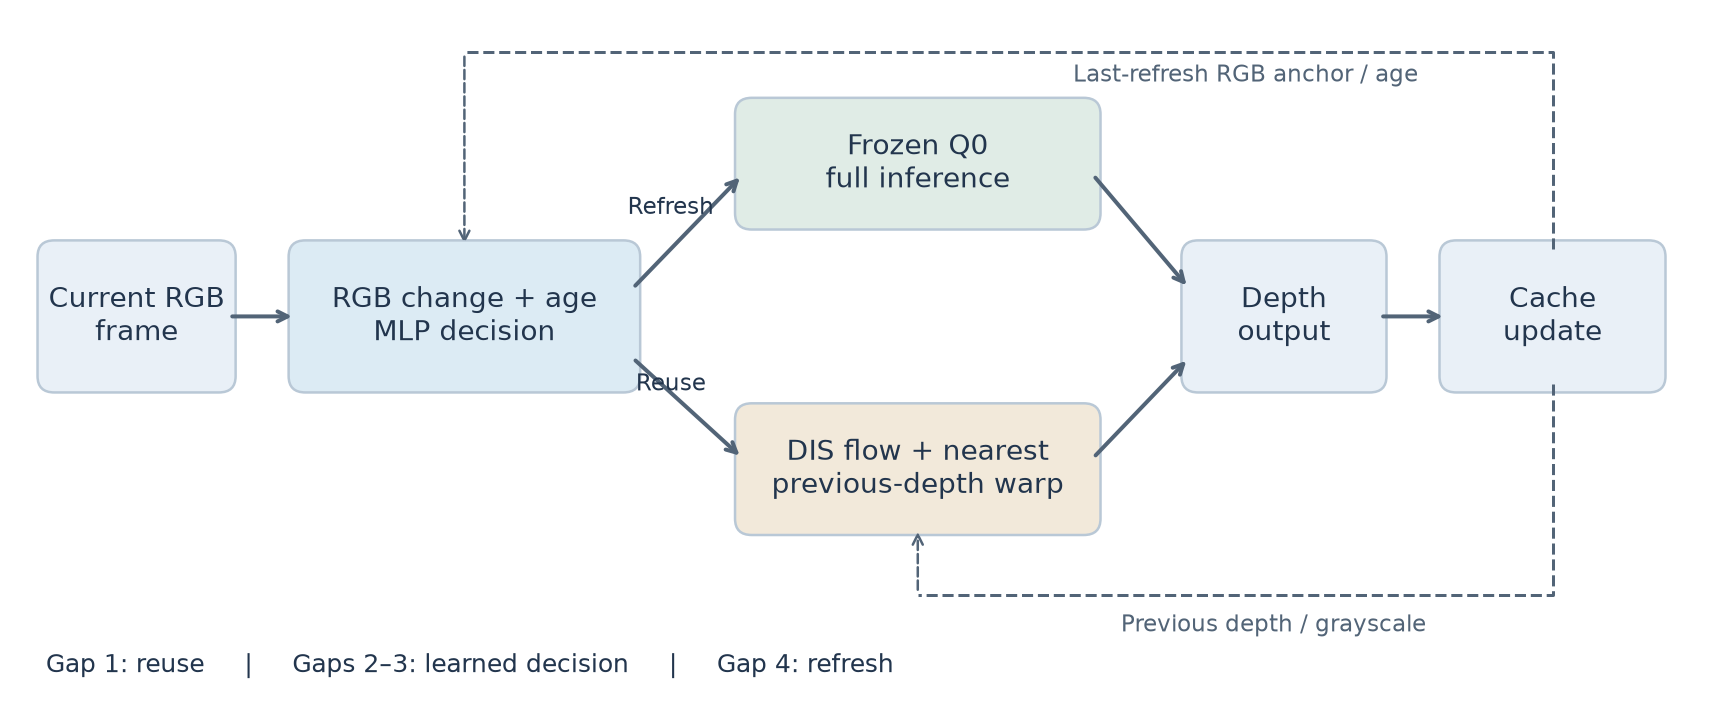
\includegraphics[keepaspectratio]{figures/architecture.png}}
\caption{Conceptual data/control flow. The RGB policy selects full Q0 inference or motion-compensated reuse. The reuse branch reads previous depth and grayscale; the policy reads anchor RGB and age. Only the selected branch runs. This is the new refresh pipeline, not the archived SSM architecture.}
\end{figure}

\subsubsection{3.2. RGB features and
policy}\label{rgb-features-and-policy}

Current and anchor RGB are bilinearly resized to 37-by-37. Their
difference contributes three channel mean absolute values and three
root-mean-square values; the current image supplies three channel means
and three standard deviations. Age divided by three and mean absolute
horizontal gradient of the RGB difference complete 14 features.

Six unused coordinates are fixed to zero, retaining the 20-dimensional
input architecture of the preceding flow-input study for comparison. Its
96 zero-coordinate input weights have zero data gradient. Normalization
statistics are fitted on policy-training data only.

The MLP uses a 20-to-16 linear layer, LayerNorm and GELU, a
16-to-39-to-16 GELU core, and scalar head. Its score is
\(s_t=0.05\operatorname{softplus}(z_t)\). This estimates a Q0
discrepancy proxy, not a calibrated failure probability or certified
error bound.

\subsubsection{3.3. Refresh and transport}\label{refresh-and-transport}

Let \(a_t\) be attempted age since the last full Q0 call. The refresh
rule is

\[
r_t=\begin{cases}
1,&\text{uninitialized or }a_t\geq4,\\
0,&a_t=1,\\
\mathbb{1}[s_t>\tau],&a_t\in\{2,3\}.
\end{cases}
\]

The frozen candidate uses \(\tau=0.05327536165714264\), the median
calibration-subset prediction. Compulsory age-one reuse means an abrupt
scene change immediately after refresh cannot trigger a new full call.
Maximum age bounds reuse duration, not its geometric error.

On refresh, \(\widehat D_t=Q(I_t)\) and age resets; rejected reuse
computes no flow. Otherwise, DIS computes both current-to-previous and
previous-to-current flow at grayscale 128-by-128, and
\(\widehat D_t=W_t(\widehat D_{t-1})\). The operator upsamples the
backward displacement and nearest-samples depth with border padding. It
does not average neighboring depth values, but incorrect correspondence
and disocclusion remain possible.

The implementation also computes a forward--backward/photometric
reliability mask. The selected ungated transport does not use that mask
to suppress or replace depth pixels; both flows and mask computation
remain included in timing. No learned residual changes the reused depth.

\subsubsection{3.4. Training and operating
points}\label{training-and-operating-points}

The training cache has 192 four-frame clips: 64 each from TUM, Bonn and
Virtual KITTI 2. Within each source, 48 clips fit the policy and 16 set
thresholds, totaling 144/48 clips. Two anchors produce 384 traces and
960 observations: 288 fit traces and 96 calibration traces, with 144
calibration observations at eligible ages two/three. Fit and calibration
frame-path sets are disjoint.

For transported candidate \(C_t\) and teacher \(D_t\), the target is

\[y_t=\|\log C_t-\log D_t\|_1+2\mathcal G(C_t,D_t),\]

where depths clamp below at \(10^{-4}\) and norms denote element means.
\(\mathcal G\) averages horizontal/vertical log-gradient discrepancies
at strides 1, 2 and 4, with weights \(1+4\min(|\nabla\log D_t|,0.25)\).
Q0 labels are training-only. They do not directly encode every GT-based
acceptance metric.

Carry SSM, per-input-reset SSM and MLP are each trained for 1,000 AdamW
steps, batch 32, learning rate .001, seed 741, with the same sampled
order and shared-layer initialization. Masked Smooth L1 compares scores
and targets divided by .05; gradient norm clips at one. SSM controls
have 1,689 parameters and MLP 1,688, but different core functions.
Thresholds are each model's calibration prediction quartiles, saved
before development inference. Selecting MLP q50 after development
comparison makes subsequent checks post-selection analyses.

\subsection{4. Conditional error and cost
analysis}\label{conditional-error-and-cost-analysis}

\subsubsection{4.1. Transport error}\label{transport-error}

For a fixed realized flow, finite-grid nearest sampling with border
replication selects one input value per output. Hence
\(\|W_t(X)-W_t(Y)\|_\infty\leq\|X-Y\|_\infty\). Define
\(e_t=\widehat D_t-D_t\) and \(b_t=W_t(D_{t-1})-D_t\). Linearity of this
fixed sampling operator gives \(e_t=W_t(e_{t-1})+b_t\) on reuse. A full
refresh at \(k\) has \(e_k=0\), yielding

\[\|e_t\|_\infty\leq\sum_{j=k+1}^{t}\|b_j\|_\infty\]

until the next refresh, by the triangle inequality and repeated
non-expansiveness. Q0 is stateless; exact refresh here does not claim to
restore a recurrent dense history.

The defects are not certified by RGB statistics or a predicted mean
log-error. Q0 itself can be wrong. No boundary-F1 or normalized flat-TV
guarantee follows. This elementary conditional analysis is a design
explanation, not a new universal stability theorem; independent
mathematical review remains pending.

\subsubsection{4.2. Paid computation}\label{paid-computation}

For identical RGB policies and deterministic flow operations, early and
late decisions have identical outputs, but late decisions additionally
compute flow on rejected reuse attempts. Under additive accounting,
early scheduling avoids that cost. With refresh fraction \(p\), a
simplified average is \(C_P+pC_Q+(1-p)C_W\), where policy/preparation,
full-Q0 and reuse costs are \(C_P,C_Q,C_W\). Reducing \(p\) helps only
if overhead and approximation remain acceptable. Actual hardware effects
require timing; skipped-call fractions are not measured speedups.

\subsection{5. Experimental protocol}\label{experimental-protocol}

\subsubsection{5.1. Data and independence}\label{data-and-independence}

L32 has eight clips/256 frames; L256 has four clips/1,024 frames. Both
cover TUM walking\_static {[}6{]} and Bonn crowd2, person\_tracking2 and
static\_close\_far {[}7{]}. Sampled frame paths do not overlap, but the
same four scenes have repeatedly informed development. These are not
independent scene-level tests. Scores average clips within scene, scenes
within source, and then the two sources equally; scenes do not receive
equal global weight.

A first local real-data audit found 28 scene directories: four reused
development scenes and 24 training-eligible scenes under the recorded Q0
setup. Training eligibility does not prove historical sampling, but
prevented certifying these remaining scenes as untouched validation. We
subsequently acquired Freiburg1 room and Freiburg2 desk from the
official TUM source after fixing the candidate. Their identifiers were
absent from the searched local training/experiment text records, and
they are separate from the recorded policy training/calibration and
reused development sequences. This establishes a new local sequence
holdout, not certified disjointness from DA2 pretraining or all possible
external history. The native-model reserved final remains unused for
this candidate. Section 6.6 reports the new holdout without threshold
retuning.

The existing numerical results below retain their original mixed-camera
status. A subsequent pose audit matched RGB timestamps to the closest
recorded camera pose within 50 ms. Its diagnostic low-motion rule
requires at least 95\% pose coverage, 95th-percentile displacement at
most 0.02 m and rotation at most 1 degree relative to the first matched
pose. Eleven of the twelve development clips exceed this motion rule;
one has insufficient coverage (93.75\%). None is certified as
fixed-mounted. For L256 walking\_static, displacement and rotation
percentiles are 0.0311 m and 2.656 degrees. Dataset names alone
therefore cannot establish fixed-camera eligibility. These diagnostic
thresholds are not accuracy guarantees; see the
\href{streaming_draft/CAMERA_POSE_AUDIT.md}{pose audit}.

For the new application, two public-data admission rounds are complete
and the depth reference is still not accepted; the second round finds
bulk values compatible with millimetres but does not establish reference
validity or registration. Eligibility requires documented fixed
mounting, usable time pairing, known metric-depth encoding and RGB/depth
registration. Foreground segmentation annotations must not be mistaken
for depth ground truth, nor may normalized depth visualization be
treated as metric depth. Sequence and location groups will be fixed
before GT evaluation; different views or clips of the same event will
not count as independent scenes. No fixed-camera GT-accuracy result is
reported yet. Section 6.7 reports a separately registered RGB-only
execution pilot.

\subsubsection{5.2. Metrics and
acceptance}\label{metrics-and-acceptance}

Raw AbsRel uses unaligned metric predictions and valid sensor GT,
excluding nonfinite GT and depths at least 150 m. Edge AbsRel uses the
GT log-depth boundary band. Boundary F1, overshoot and flat-TV follow
the preserved \texttt{sokkanaem/sharpness.py} implementation; shape
diagnostics use per-frame normalized disparity. GT fitting never changes
inference outputs. Shape diagnostics, raw metric error and temporal
consistency are distinct.

The fixed screen requires balanced raw/edge AbsRel, overshoot and
flat-TV each to increase by no more than 1\% versus Q0, boundary F1 to
drop by at most .005, and each source's raw AbsRel to increase by at
most 2\%. These are engineering tolerances, not equivalence tests or
safety certificates. Borderline failures are retained without rounding
them into passes.

\subsubsection{5.3. Timing and controls}\label{timing-and-controls}

Timing uses a shared RTX4090, batch one, GPU-resident input and
per-frame synchronization. RGB statistics, policy, CPU DIS, internal
transfers, warping and Q0 calls are included; initial I/O and input H2D
are excluded. The archived native paper's PNG-to-depth timing has a
different boundary and is not directly comparable.

Three order-rotated timing repeats follow 64 warmup frames. Controls
include dense Q0, fixed output-flow K2/K4, carry/reset SSM and MLP
quartiles, and late decisions. A sensitivity check refreshes the first
two frames before applying the unchanged selected policy, shifting
initialization by one frame.

\subsection{6. Results}\label{results}

\subsubsection{6.1. Quality retention}\label{quality-retention}

\begin{longtable}[]{@{}
  >{\raggedright\arraybackslash}p{(\linewidth - 10\tabcolsep) * \real{0.2000}}
  >{\raggedleft\arraybackslash}p{(\linewidth - 10\tabcolsep) * \real{0.1600}}
  >{\raggedleft\arraybackslash}p{(\linewidth - 10\tabcolsep) * \real{0.1600}}
  >{\raggedleft\arraybackslash}p{(\linewidth - 10\tabcolsep) * \real{0.1600}}
  >{\raggedleft\arraybackslash}p{(\linewidth - 10\tabcolsep) * \real{0.1800}}
  >{\raggedright\arraybackslash}p{(\linewidth - 10\tabcolsep) * \real{0.1400}}@{}}
\toprule\noalign{}
\begin{minipage}[b]{\linewidth}\raggedright
Data / method
\end{minipage} & \begin{minipage}[b]{\linewidth}\raggedleft
Raw AbsRel
\end{minipage} & \begin{minipage}[b]{\linewidth}\raggedleft
Edge AbsRel
\end{minipage} & \begin{minipage}[b]{\linewidth}\raggedleft
Boundary F1
\end{minipage} & \begin{minipage}[b]{\linewidth}\raggedleft
Flat-TV change
\end{minipage} & \begin{minipage}[b]{\linewidth}\raggedright
Screen
\end{minipage} \\
\midrule\noalign{}
\endhead
\bottomrule\noalign{}
\endlastfoot
L32 Q0 & .128127 & .159325 & .660219 & reference & reference \\
L32 Flow K2 & .128506 & .159792 & .662756 & +.655\% & pass \\
L32 MLP & .128377 & .160155 & .661137 & +.715\% & pass \\
L256 Q0 & .159183 & .174237 & .614665 & reference & reference \\
L256 Flow K2 & .159120 & .174638 & .620225 & +.852\% & pass \\
L256 MLP & .159336 & .174666 & .621973 & +.963\% & pass \\
\end{longtable}

Long-clip raw and edge errors rise .096\% and .246\%, while boundary F1
improves. This is retention within tolerances, not improvement of every
measure. Unrounded flat-TV growth is .963363\%, leaving only .036637
percentage points below the tolerance.

Shifted initialization passes both screens: L32/L256 raw AbsRel
.127773/.159334, F1 .663258/.621707 and flat-TV growth .309\%/.921\%.
One successful shift is not robustness to arbitrary starting times.

\subsubsection{6.2. Repeated latency}\label{repeated-latency}

\begin{longtable}[]{@{}
  >{\raggedright\arraybackslash}p{(\linewidth - 12\tabcolsep) * \real{0.1000}}
  >{\raggedleft\arraybackslash}p{(\linewidth - 12\tabcolsep) * \real{0.1200}}
  >{\raggedleft\arraybackslash}p{(\linewidth - 12\tabcolsep) * \real{0.1200}}
  >{\raggedleft\arraybackslash}p{(\linewidth - 12\tabcolsep) * \real{0.1200}}
  >{\raggedleft\arraybackslash}p{(\linewidth - 12\tabcolsep) * \real{0.1600}}
  >{\raggedleft\arraybackslash}p{(\linewidth - 12\tabcolsep) * \real{0.1800}}
  >{\raggedleft\arraybackslash}p{(\linewidth - 12\tabcolsep) * \real{0.2000}}@{}}
\toprule\noalign{}
\begin{minipage}[b]{\linewidth}\raggedright
Data
\end{minipage} & \begin{minipage}[b]{\linewidth}\raggedleft
Q0 ms
\end{minipage} & \begin{minipage}[b]{\linewidth}\raggedleft
K2 ms
\end{minipage} & \begin{minipage}[b]{\linewidth}\raggedleft
MLP ms
\end{minipage} & \begin{minipage}[b]{\linewidth}\raggedleft
Late MLP ms
\end{minipage} & \begin{minipage}[b]{\linewidth}\raggedleft
Q0 speedup
\end{minipage} & \begin{minipage}[b]{\linewidth}\raggedleft
K2 time reduction
\end{minipage} \\
\midrule\noalign{}
\endhead
\bottomrule\noalign{}
\endlastfoot
L32 & 7.491 & 4.348 & 3.720 & 3.931 & 2.014x & 14.45\% \\
L256 & 7.512 & 4.360 & 3.762 & 4.026 & 1.997x & 13.73\% \\
\end{longtable}

\begin{figure}
\centering
\pandocbounded{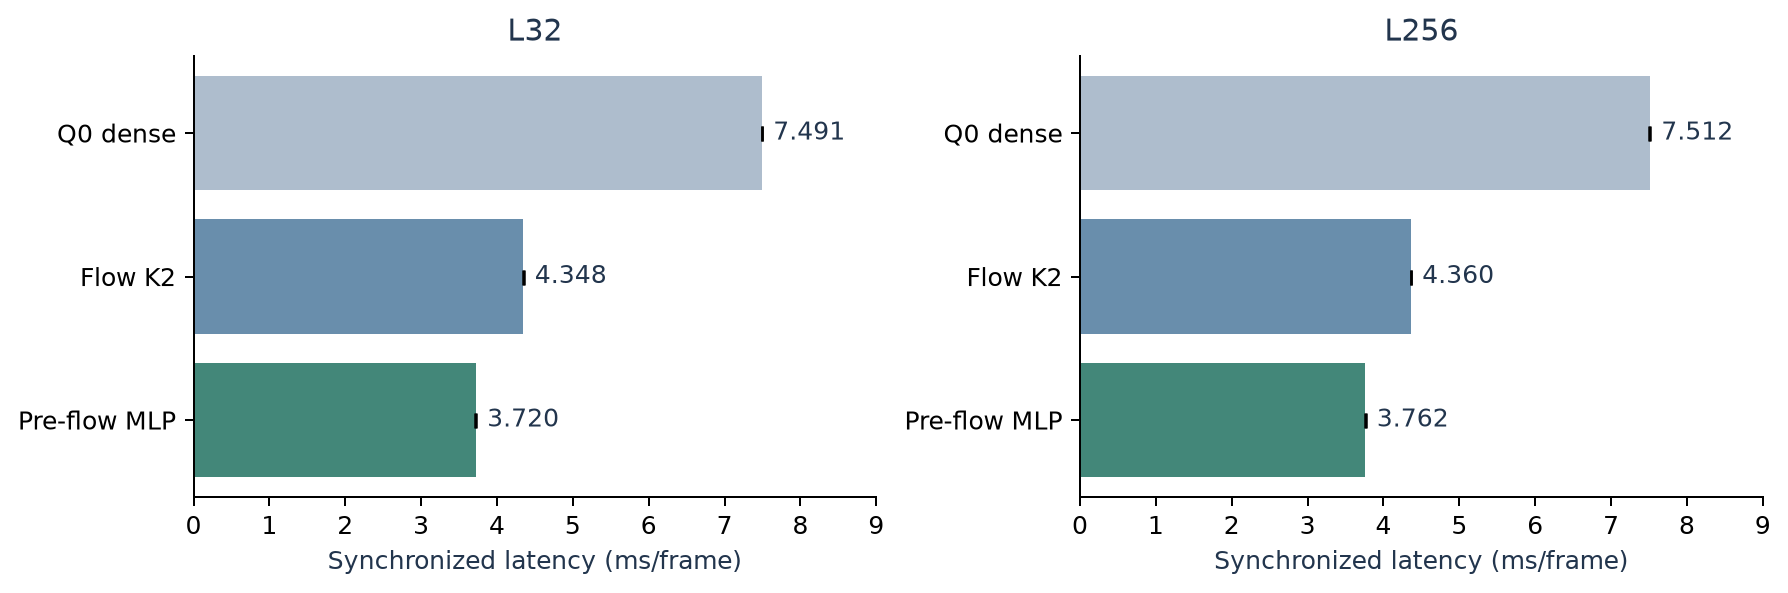
\includegraphics[keepaspectratio]{figures/latency.png}}
\caption{Three-repeat means with minimum/maximum repeat-mean error bars, not confidence intervals. MLP ranges are 3.716--3.728 ms (L32) and 3.760--3.765 ms (L256). Full-Q0 skip fractions are 62.11\% and 61.72\%. Ratios of means are not device throughput or energy measurements.}
\end{figure}

\subsubsection{6.3. Policy ablations}\label{policy-ablations}

\begin{longtable}[]{@{}
  >{\raggedright\arraybackslash}p{(\linewidth - 8\tabcolsep) * \real{0.1900}}
  >{\raggedright\arraybackslash}p{(\linewidth - 8\tabcolsep) * \real{0.2800}}
  >{\raggedright\arraybackslash}p{(\linewidth - 8\tabcolsep) * \real{0.2500}}
  >{\raggedleft\arraybackslash}p{(\linewidth - 8\tabcolsep) * \real{0.1000}}
  >{\raggedleft\arraybackslash}p{(\linewidth - 8\tabcolsep) * \real{0.1800}}@{}}
\toprule\noalign{}
\begin{minipage}[b]{\linewidth}\raggedright
Policy
\end{minipage} & \begin{minipage}[b]{\linewidth}\raggedright
L32 screen
\end{minipage} & \begin{minipage}[b]{\linewidth}\raggedright
L256 screen
\end{minipage} & \begin{minipage}[b]{\linewidth}\raggedleft
L256 skip
\end{minipage} & \begin{minipage}[b]{\linewidth}\raggedleft
L256 ms, single run
\end{minipage} \\
\midrule\noalign{}
\endhead
\bottomrule\noalign{}
\endlastfoot
Flow K2 & pass & pass & 50.00\% & 4.390 \\
Flow K4 & edge fail & edge/flat fail & 75.00\% & 2.692 \\
Carry SSM q25 & pass & pass & 53.03\% & 4.508 \\
Carry SSM q50 & edge fail & pass & 64.55\% & 3.706 \\
Carry SSM q75 & pass & edge/source fail & 69.92\% & 3.315 \\
Reset SSM q25 & pass & pass & 52.93\% & 4.508 \\
Reset SSM q50 & flat fail & pass & 63.09\% & 3.795 \\
Reset SSM q75 & edge fail & edge fail & 69.82\% & 3.325 \\
MLP q25 & pass & pass & 53.22\% & 4.371 \\
MLP q50 & pass & pass & 61.72\% & 3.791 \\
MLP q75 & raw/edge/flat/source fail & raw/edge fail & 69.63\% & 3.237 \\
\end{longtable}

No SSM operating point combines both screens and a K2 latency advantage
in both segments. MLP performance cannot be attributed to SSM memory.
Full numeric records, including late controls, are in
\texttt{streaming\_draft/evidence\_table.json}.

For identical Carry q25 on L256, early decisions reduce flow
calculations from 1,990 to 1,086: 452 rejected attempts each avoid two
flow computations. Single-run time decreases from 4.895 to 4.508 ms.
Across Carry quartiles and both lengths, early/late outputs and
schedules match on 3,840 frames. This isolates computation placement for
the same policy; older flow-input policy comparisons also change
features and training outcomes.

\subsubsection{6.4. Qualitative results and
failures}\label{qualitative-results-and-failures}

\begin{figure}
\centering
\pandocbounded{
\includegraphics[keepaspectratio]{figures/qualitative.png}}
\caption{All four L256 scenes, using the skipped MLP frame nearest each temporal midpoint, ties toward earlier frames. Depth shares 0--5 m colors, saturating above 5 m. Last column: absolute relative error against GT, saturated at .30. Gray in GT and white masked error pixels are invalid sensor locations. Cache age is shown. Similar appearance does not imply identical accuracy.}
\end{figure}

\begin{figure}
\centering
\pandocbounded{
\includegraphics[keepaspectratio]{figures/boundary_crops.png}}
\caption{Central 128-by-128 crops of Figure 3 at {[}64:192,64:192{]}. These are fixed detail views, not selected GT edge regions. Boundary evidence comes from full-image metrics.}
\end{figure}

\begin{figure}
\centering
\pandocbounded{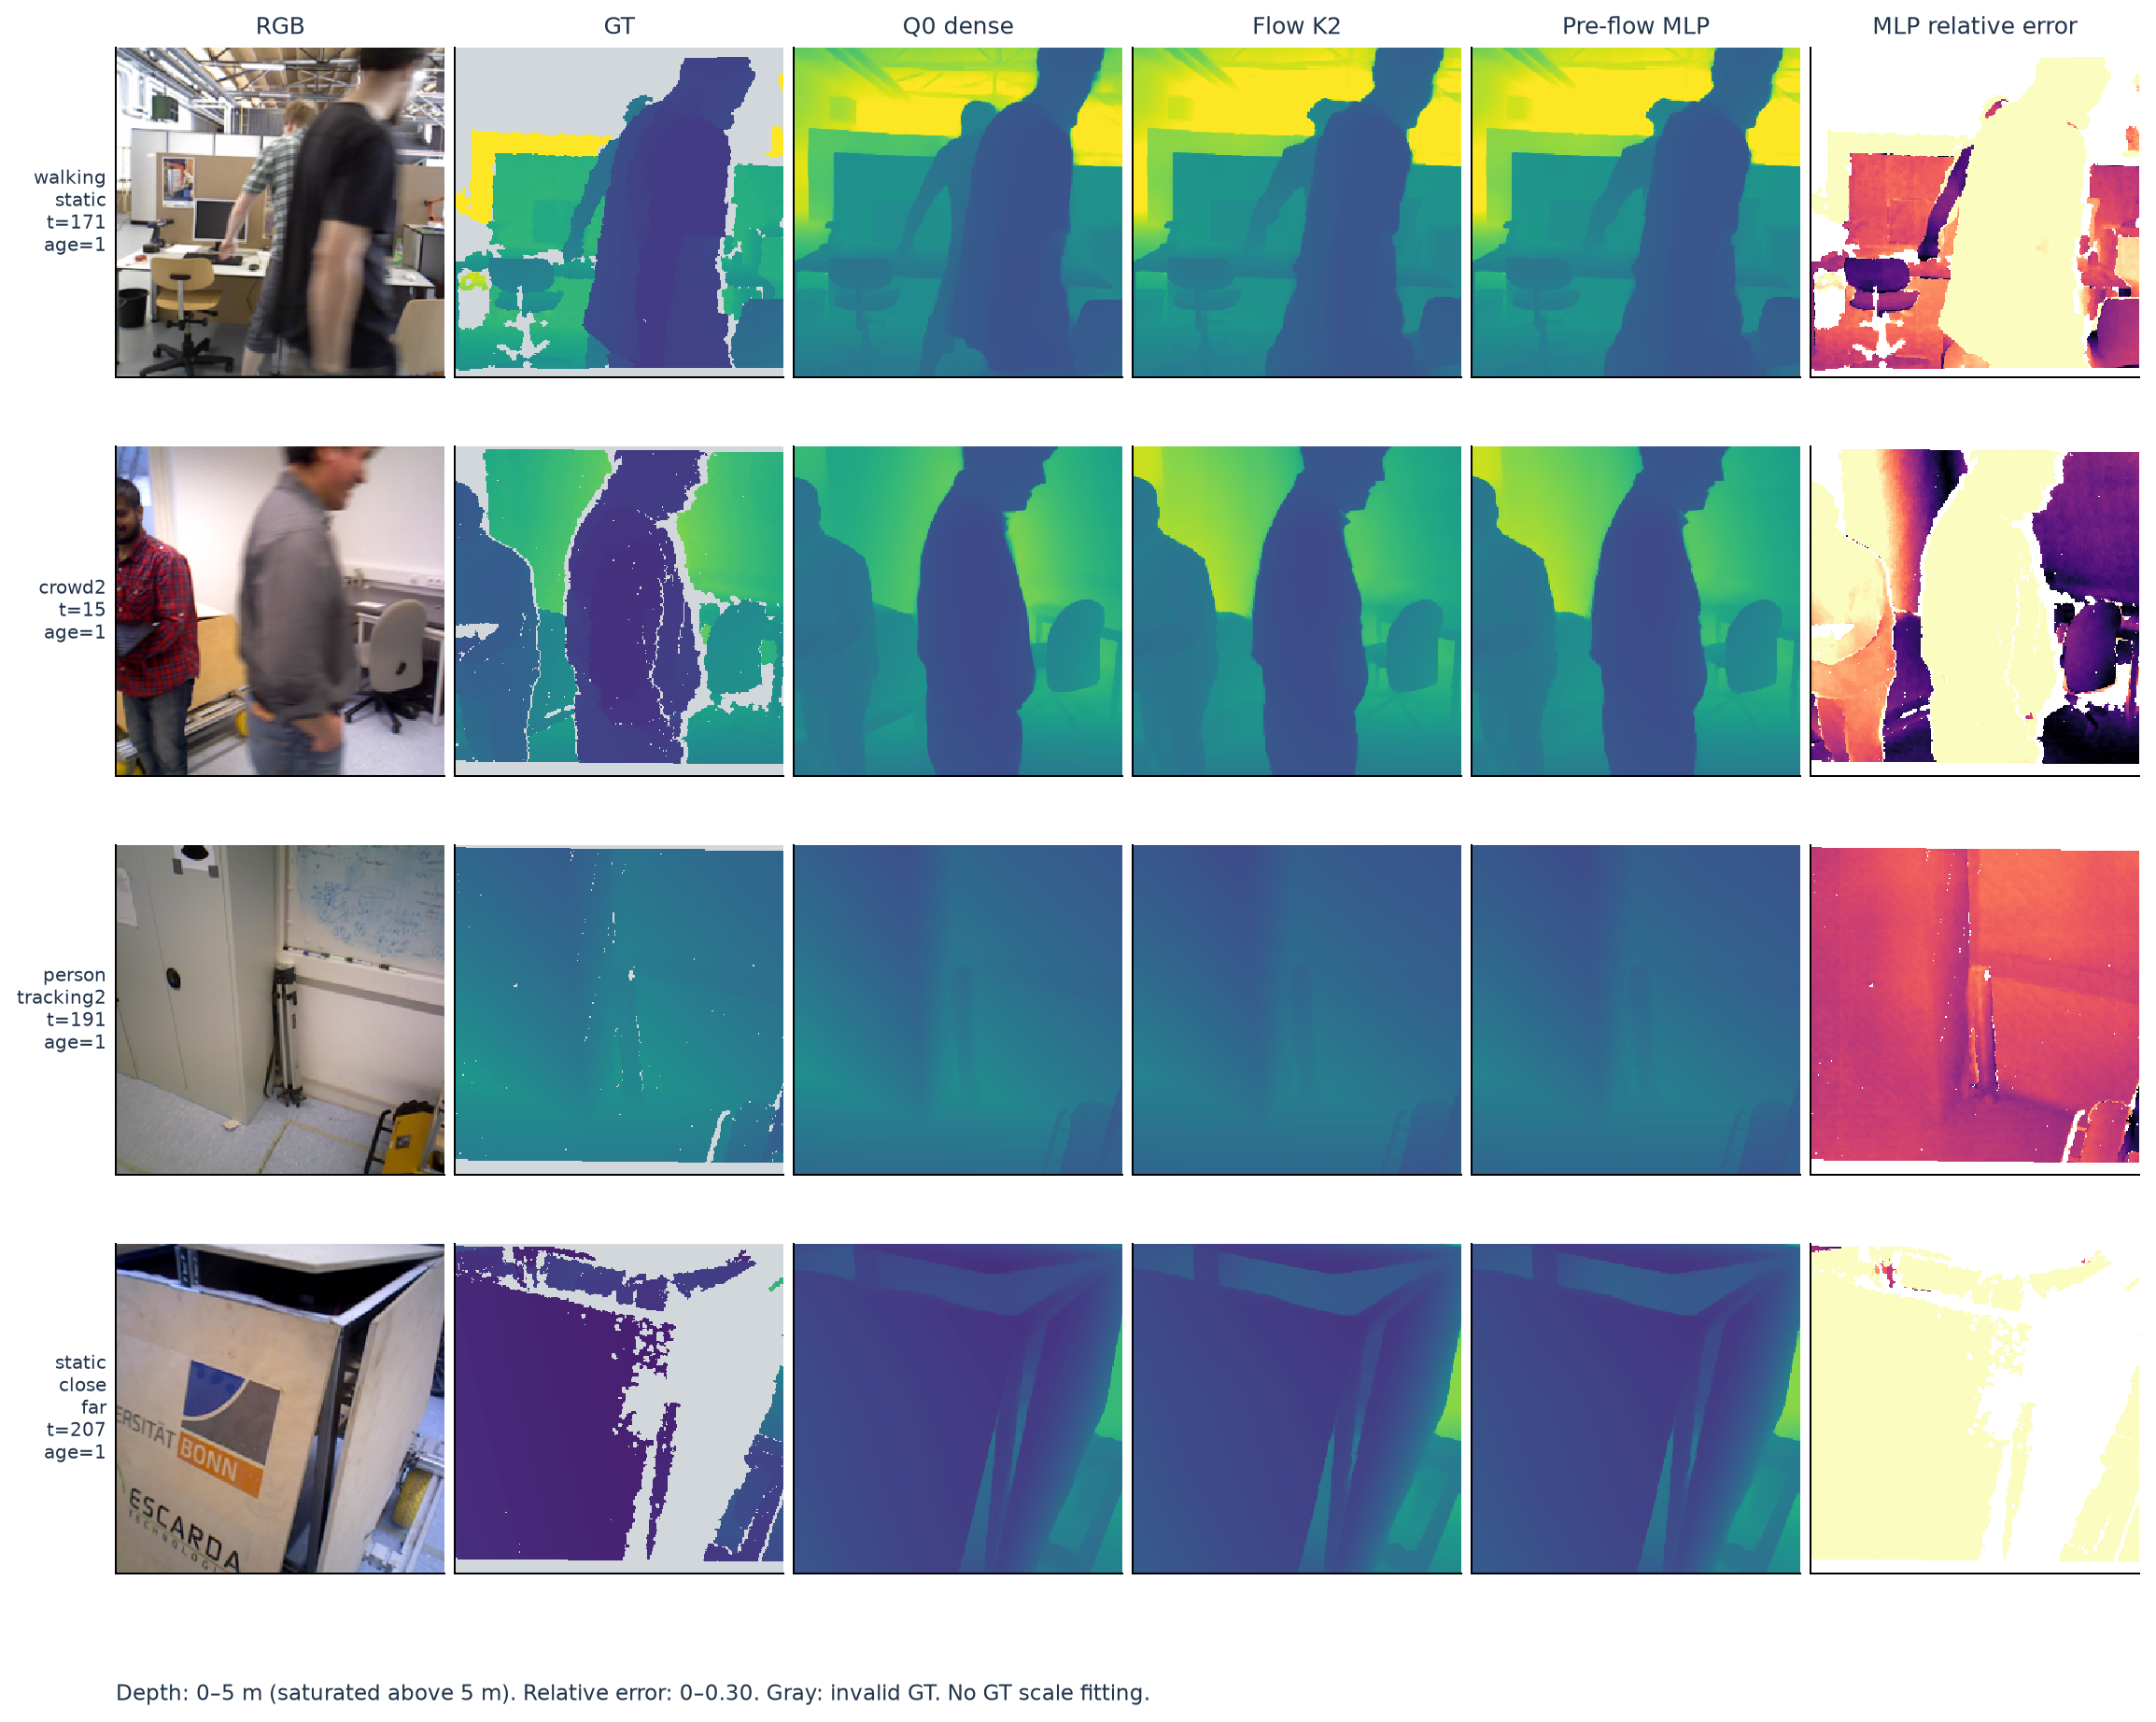
\includegraphics[keepaspectratio]{figures/failure_cases.png}}
\caption{Each scene's skipped frame with the largest per-frame raw AbsRel increase relative to Q0. This explicitly post-hoc, unfavorable selection exposes errors hidden by averages; it does not tune the frozen policy. Paths, selection rules and refresh telemetry are in streaming\_draft/visual\_provenance.json.}
\end{figure}

\subsubsection{6.5. Execution checks}\label{execution-checks}

Initial comparisons verify 6,759 full-refresh frames against Q0; shifted
initialization adds 497, totaling 7,256 exact matches. Independent
replay recomputes 9,561 learned-policy skipped outputs with exact
equality. Calibration thresholds are independently reproduced, and
code/checkpoint/input hashes remain unchanged. Related regression tests:
98 passed. These establish consistency of tested executions, not
statistical reliability on new scenes.

\subsubsection{6.6. Frozen-candidate moving-camera holdout: preserved
stress
test}\label{frozen-candidate-moving-camera-holdout-preserved-stress-test}

Before new predictions, we registered two sequences, the three methods,
the unchanged acceptance criteria and deterministic sampling. For each
sequence, L32 uses the first and last 32 timestamp-associated frames;
L256 uses 256-frame windows centered at one-third and two-thirds of the
associated timeline. The totals are 128 and 1,024 frames. Selected
RGB/depth paths do not overlap between windows. Official PNG depths are
divided by 5,000, with no additional camera-scale correction because the
released images are already corrected.

\begin{longtable}[]{@{}
  >{\raggedright\arraybackslash}p{(\linewidth - 10\tabcolsep) * \real{0.2000}}
  >{\raggedleft\arraybackslash}p{(\linewidth - 10\tabcolsep) * \real{0.1600}}
  >{\raggedleft\arraybackslash}p{(\linewidth - 10\tabcolsep) * \real{0.1600}}
  >{\raggedleft\arraybackslash}p{(\linewidth - 10\tabcolsep) * \real{0.1600}}
  >{\raggedleft\arraybackslash}p{(\linewidth - 10\tabcolsep) * \real{0.1800}}
  >{\raggedright\arraybackslash}p{(\linewidth - 10\tabcolsep) * \real{0.1400}}@{}}
\toprule\noalign{}
\begin{minipage}[b]{\linewidth}\raggedright
Data / method
\end{minipage} & \begin{minipage}[b]{\linewidth}\raggedleft
Raw AbsRel
\end{minipage} & \begin{minipage}[b]{\linewidth}\raggedleft
Boundary F1
\end{minipage} & \begin{minipage}[b]{\linewidth}\raggedleft
Overshoot change
\end{minipage} & \begin{minipage}[b]{\linewidth}\raggedleft
Flat-TV change
\end{minipage} & \begin{minipage}[b]{\linewidth}\raggedright
Screen
\end{minipage} \\
\midrule\noalign{}
\endhead
\bottomrule\noalign{}
\endlastfoot
New L32 Q0 & .283891 & .606404 & reference & reference & reference \\
New L32 K2 & .284293 & .609204 & +.557\% & +.012\% & pass \\
New L32 MLP & .284206 & .609718 & +2.285\% & +.377\% & FAIL \\
New L256 Q0 & .212614 & .583142 & reference & reference & reference \\
New L256 K2 & .212594 & .586912 & -.390\% & +.290\% & pass \\
New L256 MLP & .212941 & .587015 & -.441\% & +.363\% & pass \\
\end{longtable}

Sequence-level diagnostics reveal failures hidden by aggregation. On
short Freiburg1 room clips, overshoot grows 4.032\% for MLP and 1.593\%
for K2. On short Freiburg2 desk clips, MLP flat-TV grows 1.262\%. Both
methods pass both long-clip sequence screens. The MLP's long-clip
single-run latency is 4.260 ms versus 4.383 ms for K2 and 7.534 ms for
Q0; its K2 advantage is only 2.81\% here and has not been established by
repeated timing. Short-clip MLP is faster but fails quality, so it is
not a quality-preserving speedup.

All 1,083 full-refresh comparisons in the new experiment exactly match
Q0, and recorded weights/code/input hashes remain unchanged. The
candidate is not promoted or retuned. The report and provenance are
available in \href{streaming_draft/INDEPENDENT_VALIDATION.md}{the
new-sequence validation report}. This two-sequence holdout has now been
consumed; using these outcomes to revise the policy would make it
development data for that later model.

\subsubsection{6.7. Fixed-camera data admission and separate RGB-only
pilot}\label{fixed-camera-data-admission-and-separate-rgb-only-pilot}

We acquired the official SBM-RGBD Shadows release and its corrected
fall01cam1 depth, derived from the ceiling-mounted camera in UR Fall
Detection. The sequence has 160 contiguous RGB/depth IDs. Five complete
CRC-verified RGB files recovered from an incomplete original-archive
prefix exactly match the corresponding released RGB frames. Sparse
annotated-background feature checks support the documented fixed
mounting, but are not pose ground truth. This is one event, not multiple
independent locations.

The depth-admission check failed. Using the original published
conversion, the first original frame spans approximately 2174--3390 mm,
while the registered derivative includes positive stored values down to
1. Some values fall outside the source range in all eleven available
original-depth samples. Removing neighborhoods of zero-depth pixels does
not eliminate all such values. We do not establish whether registration,
interpolation or another processing step caused the discrepancy. We
neither fit a replacement scale to model predictions nor report GT
accuracy using this unapproved reference.

A separate predeclared RGB-only pilot processes all 160 frames
continuously with three repeats and unchanged model weights/threshold. A
minimal periodic output-hold control invokes Q0 on every second frame
and otherwise copies the previous depth, without flow or an RGB
detector. Mean resident-input times are 7.549 ms for dense Q0, 3.791 ms
for hold K2, 4.407 ms for flow K2 and 3.239 ms for MLP. The MLP makes 48
full calls, skipping 70\% of calls. Its repeated p95 range is
7.884--7.903 ms, versus 7.584--7.592 ms for Q0: mean acceleration does
not imply lower tail latency. These fixed-order shared-RTX4090
measurements exclude initial I/O/H2D and do not establish live
end-to-end real-time performance.

The complete original RGB and depth archives subsequently extended
provenance checks to all 160 frames; all RGB frames are pixel-identical
to the released inputs. Depth value agreement still fails the
prespecified criterion. A researcher-defined source-range/erosion mask
improves distributional agreement, but is not a publisher-provided
validity mask and does not verify pixelwise accuracy. Bulk values are
compatible with millimetres; this does not exclude all scale or
processing errors.

Three cross-modal registration attempts did not corroborate alignment;
the final attempt triggered its declared void condition. These failures
do not establish that alignment is impossible to test. The low-relief
statistic used in a subsequent screen depends on bin width, direction
and aggregation and is not a validated dataset-exclusion rule. A new,
separately recorded instrument check fixes histogram edges and common
support, avoids border wrap and recovers all 27 injected shifts (three
synthetic-texture cases and 24 depth self-alignment cases from eight
frames); a constant-field negative control is correctly ambiguous. This
checks known-shift localization only, not actual RGB/depth
correspondence. No admission decision is reversed. The
\href{streaming_draft/FIXED_CAMERA_REVIEW.md}{review addendum}
supersedes the broad impossibility and unit-error-exclusion
interpretations in the preserved
\href{streaming_draft/FIXED_CAMERA_REFERENCE_ADMISSION.md}{historical
admission report}.

The mean absolute relative output difference from dense Q0 is 1.800\%
for hold K2, 1.728\% for flow K2 and 2.743\% for MLP. These are
reference-retention diagnostics, not sensor-GT AbsRel and not eligible
for the GT quality gate. Sparse foreground annotations also sample
refresh phases unevenly; they cannot establish a general foreground
advantage. Across repeats, 624 full-refresh comparisons and 1,280
replayed frames match exactly. The
\href{streaming_draft/FIXED_CAMERA_VALIDATION.md}{fixed-camera
validation report} preserves the failed data admission, data-only
visualization and reproduction records. Related regression tests
including admission and minimal-hold controls: 107 passed.

\subsection{7. Discussion and
limitations}\label{discussion-and-limitations}

Fixed-view deployment is now the primary research scope, but narrowing
the scope does not repair the previously observed failures or establish
in-scope performance. Static backgrounds may dominate image-wide
averages; future evaluation must also separate moving foreground, depth
boundaries and newly revealed regions where annotations permit, and
label estimated region masks as proxies. The periodic output-hold
baseline has been implemented and timed in the RGB-only pilot; it still
needs a GT comparison alongside dense Q0, fixed-K2 flow reuse and the
learned policy to determine whether motion compensation and learned
scheduling contribute in this setting.

The improvement combines bounded reuse with sufficiently inexpensive
decisions. Expressive policy models alone do not guarantee a benefit:
conservative passing SSM policies remain slower than K2, while
unrestricted K4 reuse loses quality. Strong fixed-period controls are
essential.

Repeated use of four development scenes and post-selection auditing
permit selection bias. The subsequently registered two-sequence holdout
exposes nonuniform transfer, while pretrained-data overlap is still
unknown. The new sequence count is too small for broad statistical
generalization claims. Only one training seed and one initialization
shift are tested. Compulsory age-one reuse can miss abrupt changes;
transport cannot infer disoccluded geometry. Proxy learning does not
certify GT boundary or flat-region risk, and the original flat-TV margin
is small. A matched modern video-depth baseline, candidate-specific
motion-referenced temporal metrics, continuous long-horizon evaluation
and new Nano/Pi measurements remain absent.

The original native SSM line remains separate. Its 4.19M parameter
count, state-preservation analysis, final scores and historical hardware
evidence do not transfer to Q0-Refresh. Conversely, this pipeline's
model-path speedup does not prove acceleration of the native
architecture. Independent novelty and mathematical review are necessary
before stronger claims.

\subsection{8. Conclusion}\label{conclusion}

SOKKANAEM-Refresh targets efficient streaming depth for indoor
fixed-view cameras through pre-flow selection of full inference or
transported reuse. Historical mixed-camera development results show
approximately 14\% lower repeated mean latency than K2 within stated
quality tolerances, but the new moving-camera holdout fails short-clip
quality. These results motivate investigation; they do not yet validate
the fixed-camera application. The next requirement is a frozen-candidate
test on separately sourced, verified fixed-camera RGB-D recordings,
followed by continuous hardware end-to-end timing. Any model changes
require separate development and another fresh holdout. Neither
general-purpose quality preservation nor an SSM-memory advantage is
established.

\subsection{Reproduction and
availability}\label{reproduction-and-availability}

\texttt{streaming\_draft/frozen\_candidate.json} fixes checkpoint,
threshold and evidence. Reproduction entry points are:

\begin{itemize}
\tightlist
\item
  Training/evaluation: \texttt{scripts/qpreflow\_study.py}.
\item
  Replay: \texttt{scripts/audit\_qpreflow.py}.
\item
  Timing/phase: \texttt{scripts/audit\_qpreflow\_candidate.py}.
\item
  Assets and local split audit:
  \texttt{scripts/prepare\_streaming\_draft.py}.
\item
  Figure 1 layout refinement:
  \texttt{scripts/refine\_streaming\_layout.py}.
\item
  Camera-pose audit: \texttt{scripts/audit\_camera\_pose.py}.
\end{itemize}

The \href{streaming_draft/FIXED_CAMERA_SCOPE.md}{fixed-camera scope},
\href{streaming_draft/PUBLIC_DATASET_SCREENING.md}{public-data screening
record} and subsequent
\href{streaming_draft/FIXED_CAMERA_VALIDATION.md}{admission/pilot
report} distinguish the new target from completed historical
experiments. Public source documentation is available for
\href{https://fenix.ur.edu.pl/~mkepski/ds/uf.html}{URFD} and
\href{https://rgbd2017.na.icar.cnr.it/SBM-RGBDdataset.html}{SBM-RGBD}.
Data and RGB-only pilot entry points are
\texttt{scripts/admit\_fixed\_camera\_sbm.py},
\texttt{scripts/diagnose\_fixed\_depth.py} and
\texttt{scripts/benchmark\_fixed\_rgb.py}. The second admission round
against the complete original reference uses
\texttt{scripts/admit\_fixed\_camera\_urfd.py},
\texttt{scripts/audit\_fixed\_camera\_registration.py} and
\texttt{scripts/audit\_fixed\_camera\_registration2.py}. The hardware
objective is sustained 30-frame/s input, assessed using end-to-end
mean/p95 latency, 33.3 ms deadline exceedance and backlog/dropped
frames. Current resident-input RTX 4090 timings do not establish this
objective on Jetson Nano B01 or Raspberry Pi 4.

The preserved scorer supplies exact diagnostic thresholds and
normalization. Public release, dataset/weight redistribution rights and
author approval remain unconfirmed.

\subsection{References}\label{references}

\begin{enumerate}
\def\labelenumi{\arabic{enumi}.}
\tightlist
\item
  Yang, L., et al.~Depth Anything V2. 2024.
  \href{https://arxiv.org/abs/2406.09414}{Paper}.
\item
  Kroeger, T., et al.~Fast Optical Flow using Dense Inverse Search.
  2016. \href{https://arxiv.org/abs/1603.03590}{Paper}.
\item
  Dutson, M.; Li, Y.; Gupta, M. Eventful Transformers: Leveraging
  Temporal Redundancy in Vision Transformers. 2023.
  \href{https://arxiv.org/abs/2308.13494}{Paper}.
\item
  Chen, S., et al.~Video Depth Anything: Consistent Depth Estimation for
  Super-Long Videos. 2025.
  \href{https://arxiv.org/abs/2501.12375}{Paper}.
\item
  Online Video Depth Anything: Temporally-Consistent Depth Prediction
  with Low Memory Consumption. 2025.
  \href{https://arxiv.org/abs/2510.09182}{Paper}.
\item
  TUM RGB-D benchmark dataset documentation.
  \href{https://cvg.cit.tum.de/data/datasets/rgbd-dataset}{Dataset}.
\item
  Bonn RGB-D Dynamic Dataset.
  \href{https://www.ipb.uni-bonn.de/data/rgbd-dynamic-dataset/}{Dataset}.
\end{enumerate}

Full reference metadata, dataset citations in context, related-work
completeness and journal-specific formatting require a final
bibliographic pass before submission.

\end{document}
